\begin{figure*}[t]
\centering
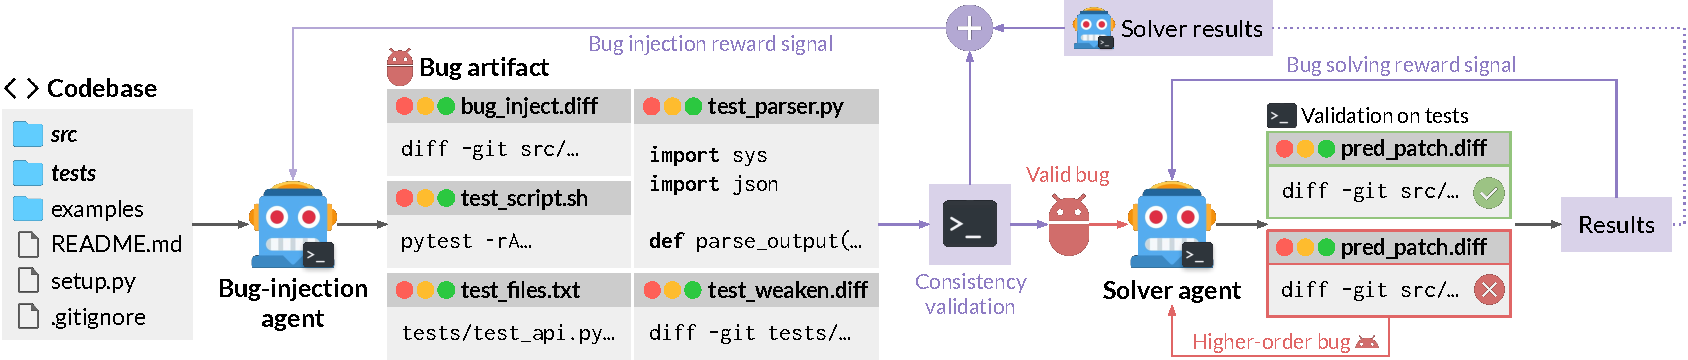
\includegraphics[width=\linewidth]{plots/ssr-overview.pdf}
\caption{Overview of \techfull{}.}
\label{fig:overview}
\end{figure*}


\section{Introduction}
\label{section:intro}

Software engineering agents~\cite{yang2024sweagent,wang2024openhands,moatless,zhang2024autocoderover,xia2024agentless,xia2025livesweagentsoftwareengineeringagents,zhang2025darwin,deepswe2025,yang2025kimidevagentlesstrainingskill,faircodegenteam2025cwmopenweightsllmresearch,seed2025seed-oss,devstral} based on large language models (LLMs) have advanced rapidly and are boosting developer productivity in practice~\cite{index2025airoi}.
To improve LLMs' agentic ability, reinforcement learning (RL) with verifiable rewards has become the focal point.
SWE-RL~\cite{wei2025swerl} is the first open RL method to improve LLMs on software engineering tasks using rule-based rewards and open software data. Since then, a variety of open LLMs focused on agentic RL have been released, including DeepSWE~\cite{deepswe2025}, DeepSeek V3.1~\cite{deepseekv31}, MiniMax M1/M2~\cite{chen2025minimax}, Kimi K2~\cite{kimiteam2025kimik2openagentic}, and Code World Model~\cite{faircodegenteam2025cwmopenweightsllmresearch}.
However, both the data and the environments used to train these agents, such as the issue descriptions and test cases, are heavily based on human knowledge or annotations.
Even with RL applied, the resulting agents primarily learn to replay and refine human software development traces rather than independently discovering new classes of problems and solutions. 
Moreover, such curated training signals can be unreliable without extensive human inspection, as evidenced by the need for human-verified evaluation subsets like \sbv~\cite{swebverified}.
Consequently, this dependence on human knowledge and curation is unlikely to scale indefinitely, making it difficult for software agents to achieve the open-ended or superintelligent capabilities that purely self-improving systems might attain.

Although recent efforts such as SWE-smith~\cite{yang2025swe} and BugPilot~\cite{sonwane2025bugpilotcomplexbuggeneration} explore the use of LLMs for large-scale synthetic bug generation, these methods often hold stronger human-data assumptions, such as access to test suites and parsers, thus suffering the same aforementioned scalability limitations, and depend on teacher models for distillation.
In addition, such existing methods typically rely on static bug generation pipelines without any consideration of the model being trained, limiting their ability to generate maximally informative examples as the agent improves.
As a result, the system cannot continually self-improve.

In contrast, some of the most compelling examples of superintelligent AI arise from self-play.
Following AlphaGo~\cite{silver2016mastering}, AlphaZero~\cite{alphazero} achieves self-improvement in Go, chess, and shogi through self-play with only the game rules as input, showing that exploring and exploiting the implications of these game rules using RL can reach superhuman play.
Recently, researchers have started to adopt self-play in open domains~\cite{zhao2025absolutezeroreinforcedselfplay,
huang2025rzeroselfevolvingreasoningllm,
kuba2025languageselfplaydatafreetraining,
lin2025learningsolveverifyselfplay,
chen2025selfquestioninglanguagemodels,
liu2025rstarcoderscalingcompetitivecode,
haluptzok2023languagemodelsteachprogram}, some impressively but implausibly using nearly zero external data and relying on LLM introspection instead.
Absolute Zero~\cite{zhao2025absolutezeroreinforcedselfplay} trains a single reasoning model to propose coding tasks that maximize its own learning progress and improves reasoning by solving them.
Similarly, R-Zero~\cite{huang2025rzeroselfevolvingreasoningllm} co-evolves a challenger and a solver to improve LLMs' reasoning on multiple domains.
LSP~\cite{kuba2025languageselfplaydatafreetraining} also shows that pure self-play can enhance LLMs' instruction-following capability.
However, such ``zero'' self-play cannot acquire knowledge beyond the fixed environment rules and the model's existing knowledge. Instead, SPICE~\cite{spiceselfplay} performs corpus-grounded self-play to interact with the external world for diverse feedback, which improves LLMs' general reasoning ability and outperforms ungrounded methods. For a thought experiment, consider what a human can learn by only interacting with the Python interpreter like in Absolute Zero.
While they can learn all the intricacies of Python, they cannot learn the much greater knowledge and experiences contained in real-world codebases not inferable from Python semantics.
This raises a natural question for software engineering: can we build software agents that, grounded in extensive real-world repositories, learn primarily from their own interaction with diverse code environments rather than from human-curated training data?

Inspired by these developments, we propose \techfull (\tech), a first step toward superintelligent software engineering agents that learn from their own experience grounded by raw codebases.
\tech assumes only access to a corpus of sandboxed environments, each containing the source repository and its dependencies, without any knowledge about existing tests, test runners, issue descriptions, or language-specific infrastructure.
In practice, each input to \tech consists solely of a pre-built Docker image.
As shown in \cref{fig:overview},
a single LLM policy is instantiated in two roles by different prompting: a bug-injection agent and a bug-solving agent, both having access to the same set of tools adapted from Code World Model (\cwm)~\cite{faircodegenteam2025cwmopenweightsllmresearch}, including Bash and an editor.
When the model plays the bug-injection role, it explores the repository, discovers how to run tests, and constructs a \emph{bug artifact} that formally specifies a bug via a standard suite of artifacts: (1) a bug-inducing patch over code files, (2) a test script, (3) test files, (4) a test parser script, and (5) a test-weakening patch over test files. These artifacts are validated through a series of consistency checks and then handed to the solver role. Then the model plays the solver role, where it sees only the reversed test-weakening patch as a formal specification of the required behavior and must produce a repair patch that satisfies all specified tests. Both roles share parameters and are trained jointly with RL.
We further introduce \emph{higher-order bugs} constructed from the solver’s own failed repair attempts. They enrich the training distribution by exposing the system to  increasingly layered and realistic failure patterns that resemble the multi-step, interdependent edits required in real-world software development.
Through comprehensive self-play, the model itself can generate an evolving curriculum of diverse, challenging bugs that naturally reflects its online and changing policy,
which static bug-generation pipelines cannot provide.

We evaluate \tech on the widely-used \sbv benchmark~\cite{swebench,swebverified} and the more complex \sbp benchmark~\cite{deng2025swebenchproaiagents} using \cwm-sft---the pre-RL checkpoint of \cwm---as the base model.
Our results indicate that \tech consistently surpasses the ``human-data'' baseline on both benchmarks over the entire training trajectory. This baseline is trained with the same hyperparameters as \tech and uses the same environment images, but it receives human-authored or human-curated issue descriptions together with the corresponding test suites and test commands for reward computation, following the setting of \cwm’s agentic SWE-RL training.
Furthermore, our results show that while self-play is effective across various bug-injection strategies, the choice of strategy introduces subtle but meaningful differences in training effectiveness. Vanilla bug-injection prompting causes the injected bugs to collapse into superficial one-line modifications, yielding weak learning signals. Conversely, encouraging aggressive code removals and leveraging insights from historical changes improve the quality and effectiveness of learning.
Finally, we demonstrate that self-play training provides superior performance compared with repair-only training, which conducts RL exclusively on bugs proposed by the proposer from earlier self-play iterations without engaging in new bug generation.

Overall, \techfull suggests a first step toward superintelligent software agents that autonomously accumulate vast learning experience from software repositories, eventually enabling systems that surpass human capabilities in understanding, improving, and generating software.

\textbf{Conflict of Interest Disclosure.} Several authors of this paper are employed by Meta, which leads the development of Code World Model (CWM)~\cite{faircodegenteam2025cwmopenweightsllmresearch} and CWM-sft~\cite{cwmsft}, which are used as the base model and comparison points evaluated in this paper. The work also uses infrastructure and environment images associated with CWM.




